\documentclass[aspectratio=169]{beamer}


\usetheme[compress]{Drexel}

\author[S.~Lewis]{Sean Lewis}
\date[2018-28-08]{August 28, 2018}
\title[Progress Report]{\Huge Summer Research: \\ Hypervelocity Globular Cluster}
\institute{Drexel University}

\begin{document}

\begin{frame}
  \maketitle
\end{frame}

\section{HVGC-1}
\subsection{HVGC-1}

\begin{frame}
  {HVGC-1 Radial and Tangential Velocity}
  \begin{itemize}
    \item HVGC-1 observed to have 2300 km/s radial velocity towards earth. 
    \item Tangentially removed from M87 by 85 kpc. 
    \item Must have some tangential velocity component (probably small compared to radial velocity less the object is more extraordinary than it already is).
    \item Tangential velocity determines how long HVGC-1 has been traveling. We are limited here as M87 is 16.4 Mpc away and observations assumed HVGC-1 was also 16 Mpc away.
  \end{itemize}
  
\end{frame}

\begin{frame}
  {Necessary Ejection Velocities}
  \begin{columns}
    \column{0.5\textwidth}
    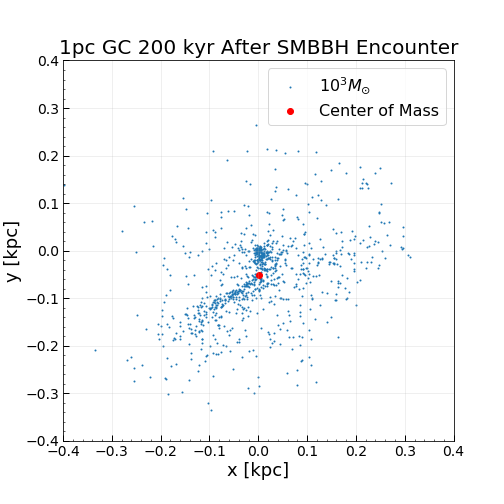
\includegraphics[width=6.4cm, height=6.4cm]{./Images/1pc200kyr_scatter.png}
    \centering
    \column{0.5\textwidth}
    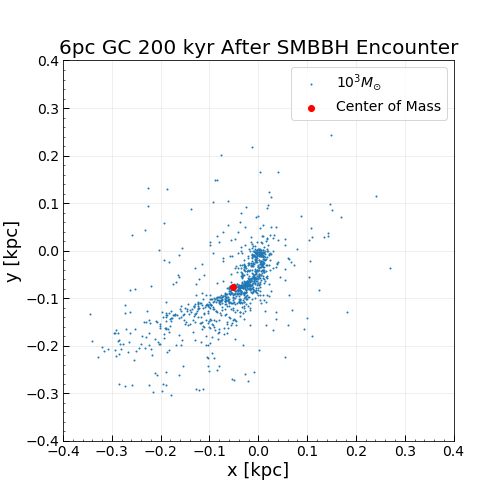
\includegraphics[width=6.4cm, height=6.4cm]{./Images/6pc200kyr_scatter.png}
    \centering
  \end{columns}
\end{frame}

\begin{frame}
  {Necessary Ejection Velocities}
  \begin{columns}
    \column{0.5\textwidth}
    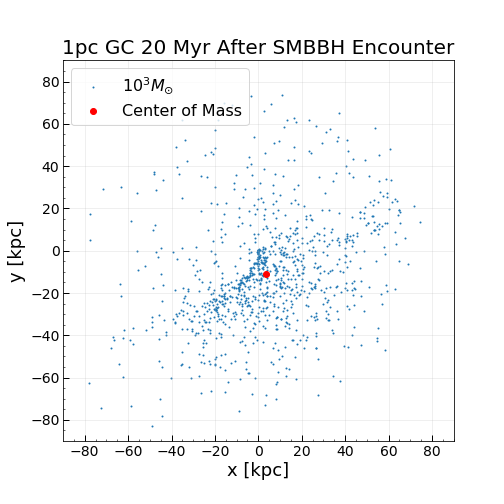
\includegraphics[width=6.4cm, height=6.4cm]{./Images/1pc20Myr_scatter.png}
    \centering
    \column{0.5\textwidth}
    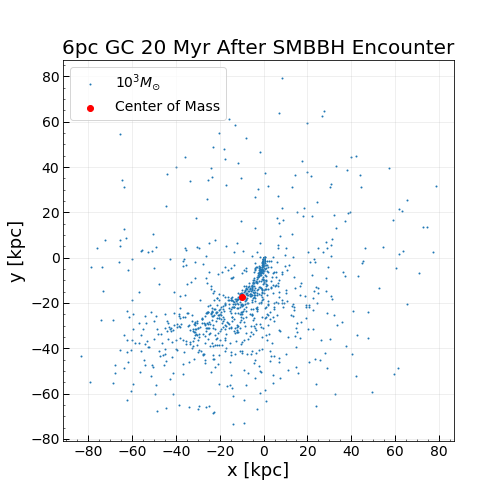
\includegraphics[width=6.4cm, height=6.4cm]{./Images/6pc20Myr_scatter.png}
    \centering
  \end{columns}
\end{frame}

\begin{frame}
  {Necessary Ejection Velocities}
  \begin{columns}
    \column{0.5\textwidth}
    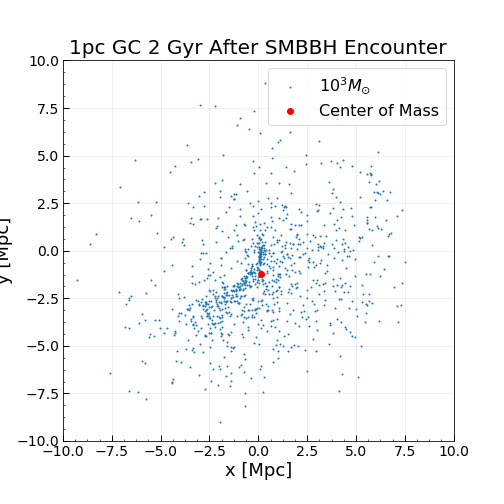
\includegraphics[width=6.4cm, height=6.4cm]{./Images/1pc2Gyr_scatter.png}
    \centering
    \column{0.5\textwidth}
    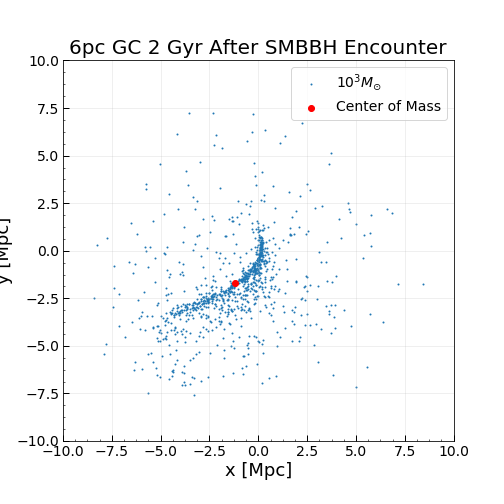
\includegraphics[width=6.4cm, height=6.4cm]{./Images/6pc2Gyr_scatter.png}
    \centering
  \end{columns}
\end{frame}

\backupbegin

\begin{frame}
  {}
  \begin{center}
    \Huge Backup Slides
  \end{center}
\end{frame}

\subsection{}
\begin{frame}
  {3:1 Mass ratio}
  \begin{columns}
    \column{0.5\textwidth}
    \begin{itemize}
      \item 2-3 pc pass from larger BH.
      \item Tidal radius of 0.3-0.4 pc
    \end{itemize}
    \column{0.6\textwidth}
    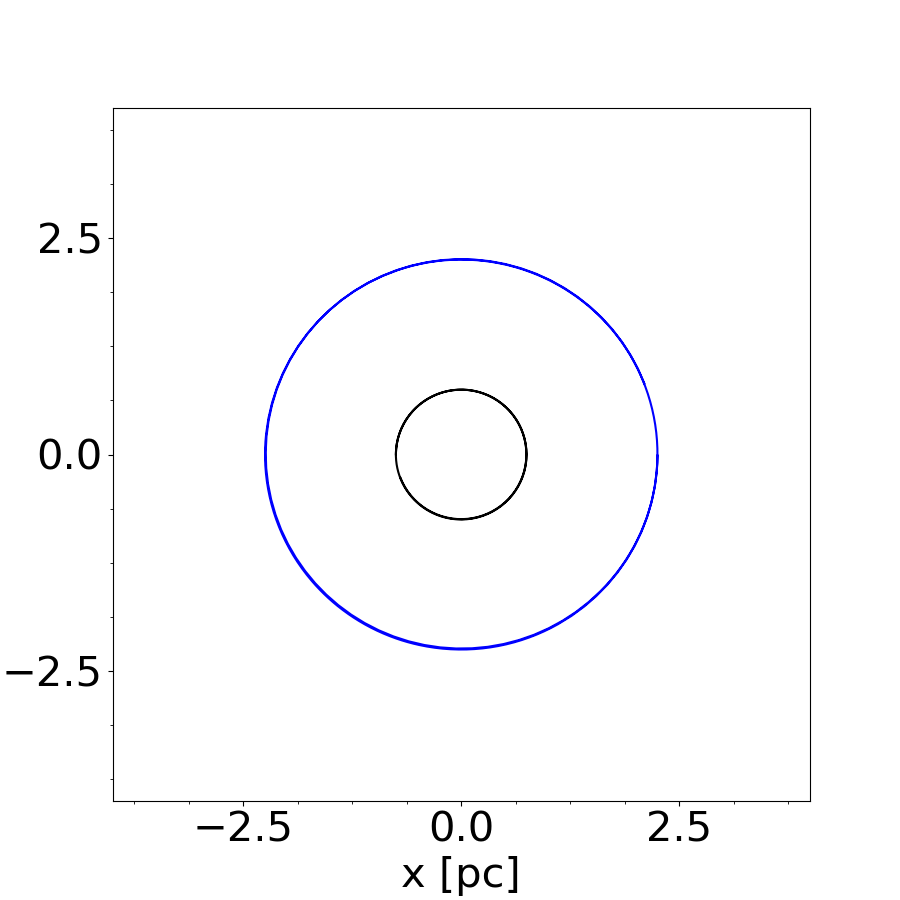
\includegraphics[width=6cm, height=6cm]{./Images/hvgc1_0333ratio.png}
    \centering
  \end{columns}
\end{frame}

\backupend
\end{document}